\documentclass[a4,useAMS,usenatbib,usegraphicx]{mn2e} 
%=========================================================================
\usepackage{amsmath} 
\usepackage{amssymb} 
\usepackage {graphicx}
\usepackage[dvips]{epsfig}
\usepackage{epsfig}  
\usepackage{color}
\usepackage[normalem]{ulem}
\usepackage{hyperref}
\usepackage{caption}
%Non reposionated tables
\usepackage{float}
\restylefloat{table}
%Multiple columns support for tables
\usepackage{array}
\usepackage{booktabs}
\setlength{\heavyrulewidth}{1.5pt}
\setlength{\abovetopsep}{4pt}


%=========================================================================
%		INTERNAL MACROS
%=========================================================================
\def\be{\begin{equation}}
\def\ee{\end{equation}}
\def\ba{\begin{eqnarray}}
\def\ea{\end{eqnarray}}

% To highlight comments 
\definecolor{red}{rgb}{1,0.0,0.0}
\newcommand{\red}{\color{red}}
\definecolor{darkgreen}{rgb}{0.0,0.5,0.0}
\newcommand{\SRK}[1]{\textcolor{darkgreen}{\bf SRK: \textit{#1}}}
\newcommand{\SRKED}[1]{\textcolor{darkgreen}{\bf #1}}
\newcommand{\before}[1]{\textcolor{red}{ #1}}
\newcommand{\after}[1]{\textcolor{darkgreen}{ #1}}

\newcommand{\tol}{Tololo 1214-277}
\newcommand{\lya}{Ly$\alpha$}
\newcommand{\hb}{H$\beta$}
\newcommand{\ha}{H$\alpha$}
\newcommand{\oiii}{[OIII]}
\newcommand{\oii}{[OII]}
\newcommand{\nii}{[NII]}
\newcommand{\esca}{erg cm$^{-2}$ s$^{-1}$ \AA$^{-1}$}
\newcommand{\esc}{erg cm$^{-2}$ s$^{-1}$}
\newcommand{\es}{erg s$^{-1}$}
\newcommand{\esa}{erg s$^{-1}$}
\newcommand{\kms}{km s$^{-1}$}
\newcommand{\apj}{ApJ}  
\newcommand{\jcap}{JCAP}  
\newcommand{\apjs}{ApJS}  
\newcommand{\pasa}{PASA}  
\newcommand{\apjl}{ApJL}  
\newcommand{\aj}{AJ}  
\newcommand{\mnras}{MNRAS}  
\newcommand{\mnrassub}{MNRAS accepted}  
\newcommand{\aap}{A\&A}  
\newcommand{\aaps}{A\&AS}  
\newcommand{\araa}{ARA\&A}  
\newcommand{\nat}{Nature}  
\newcommand{\physrep}{PhR}
\newcommand{\pasp}{PASP}    
\newcommand{\pasj}{PASJ}    
\newcommand{\sigmaclump}{$54.3\pm 0.6$ km s$^{-1}$}
\newcommand{\inftyclump}{$54.3\pm 5.1$ km s$^{-1}$}
\newcommand{\probaclump}{$0.96\pm 0.01$}
\def\simgt{\lower.5ex\hbox{\gtsima}}
\def\simlt{\lower.5ex\hbox{\ltsima}}

\begin{document}

%=========================================================================
%		FRONT MATTER
%=========================================================================
\title[An atypical Lyman-$\alpha$ dwarf galaxy]{
Clumpiness and rotation: possible causes for an atypical Lyman-$\alpha$ dwarf galaxy}
\author[J.E. Forero-Romero et al.]
{Jaime E. Forero-Romero $^{1}$ \thanks{je.forero@uniandes.edu.co},
Max Gronke$^2$, 
Mar\'ia Camila Remolina-Guti\'errez$^1$,
\newauthor
Nicol\'as Garavito-Camargo$^3$, 
Mark Dijkstra$^2$\\
%%
$^1$ Departamento de F\'isica, Universidad de los Andes, Cra. 1
  No. 18A-10 Edificio Ip, CP 111711, Bogot\'a, Colombia \\
$^2$ Institute of Theoretical Astrophysics, University of Oslo,
Postboks 1029 Blindern, NO-0315 Oslo, Norway.\\
$^3$ Department of Astronomy, University of Arizona, 933 North Cherry
Avenue, Tucson, AZ 85721, USA. 
}

%\vspace*{6pt}\\

%}
\maketitle


\begin{abstract}
  Star-forming Compact Dwarf Galaxies (CDGs) resemble the expected
  pristine conditions of the first galaxies in the Universe.    
Before the observational detection of the first galaxies becomes
reality, CDGs are the best systems to test our ideas on primordial
galaxy formation and evolution.    
Here we report on one of such CDGs, \tol, which presents
a broad symmetric Lyman-$\alpha$ line emission that had evaded theoretical
interpretation so far. 
In this paper we explain these features by two different models: 
an interstellar medium composed by outflowing clumps with additional
random motions and an homogeneous gaseous sphere undergoing bulk rotation.
It is the first time that an observed \lya\ spectrum can be explained
assuming either of these physical conditions.
We find that both models independently require high velocities
(either a  a clump velocity dispersion of \sigmaclump\ with outflows of
\inftyclump\ or a bulk rotation of $348^{+75}_{-48}$ km s$^{-1}$)
consistent with a dynamical mass of at 
least a $10^{10}$ M$_{\odot}$, ten times larger than its baryonic mass.   
We argue that a possible explanation for this excess of
dynamical mass is the presence of a supermassive black hole at the
center of \tol. 
This work demonstrates the importance of considering multiphase
physics and rotation among the possible conditions shaping the
\lya\ spectra of the first galaxies.  
Additionally, if future kinematic maps of \tol\ confirm the high
velocities postulated in our model, it would provide new
evidence for dwarf galaxies as hosts of supermassive black
holes.  
\end{abstract}

\begin{keywords}
Methods: data analysis - numerical 
\end{keywords}


%=========================================================================
%		PAPER CONTENT
%=========================================================================

%*************************************************************************
\section{Introduction}
\label{sec:introduction}





Primordial galaxies have not been detected yet. 
However, dwarf star forming galaxies with a low metallicity content
are seen as templates to understand the early galaxy evolution process. 
Almost fifty years ago \citep{PartridgePeebles} it was realized that
young galaxies could be detected through a strong Lyman-$\alpha$ line
emission.  


This theoretical prediction was only confirmed thirty years later on
distant, relatively young, not primordial, galaxies \citep{1998ApJ...498L..93D}.
Currently Lyman Alpha Emitting (LAE) galaxies are commonly targeted
in surveys. 
The presence of the Ly-$\alpha$ emission line provides confirmation of
the distance of a galaxy while provides clues about the stellar
population and inter-stellar medium conditions regulating the
Ly-$\alpha$ emission. 

The Ly-$\alpha$ emission line is not exclusive of distant galaxies. 
Any galaxy with low dust content and ongoing star formation has the
right conditions to show this line.  
There are, for instance,  local Universe surveys that target
Ly-$\alpha$ emission in nearby dwarf star forming galaxies 
\citep{LARS}. 
The study of nearby LAE samples has allowed the study of other
indicators that might be more difficult to obtain for distant galaxies
such as morphology, dust attenuation, neutral hydrogen contents and
ionization state.  

However, the physical interpretation of Ly-$\alpha$ observations is
not straightforward \citep{2015ApJ...805...14R}. 
This is due to the resonant nature of the Ly-$\alpha$ line. 
A Ly-$\alpha$ photon follows a diffusion-like process before escaping
the galaxy or being absorbed by dust. 
The resulting line profile becomes sensitive to the dynamical, chemical
and thermal conditions in the interstellar medium. 
There are very few analytically tools available to interpret the
emerging Ly-$\alpha$ line.
They are applicable only in very few cases of highly symmetrical
conditions, which are hardly met in real astrophysical systems.
For these reasons the interpretation of Ly-$\alpha$ observations
requires state-of-the-art Monte Carlo radiative transfer simulations.   

\tol\ is a compact star forming dwarf galaxy that presents a
strong Ly-$\alpha$ emission \citep{Thuan97} with two puzzling 
features: the line is symmetric and single peaked.
Usually the Ly-$\alpha$ line has an asymmetric single or double peak. 
These two special features in \tol\ cannot be explained with
conventional models \citep{2006A&A...460..397V,2015ApJ...812..123G}.  

In this paper we show how the \tol's \lya\ profile can be explained
either by  or the recently developed class of complex multiphase models 
\citep{Gronke2016} or by a simple rotation model
\citep{GaravitoCamargo2014}. 
\section{Observations}


\tol's basic observational characteristics are summarized in Table \ref{obstable}.
Its receding velocity is $7785\pm 50$km s$^{-1}$, which translates
into a distance of $106.6$ Mpc (with the Hubble constant $H_{0}$=73
Mpc km s$^{-1}$) 



The observed flux for the Lyman alpha line is $\sim
8.1\times 10^{-14}$ erg cm$^{-2}$ s$^{-1}$ \citep{Thuan97}
and a Equivalent Width of $70$\AA\ and its H$\beta$ flux is 
$1.62\times 10^{-14}$ erg cm$^{-2}$ s$^{-1}$ \AA${-1}$
\citep{Izotov04} which gives a Ly$\alpha$/H$\beta$ flux ratio of
4.9$\pm$0.1. The Ly-$\alpha$ flux values correspond to luminosities of
$L_{Ly\alpha}=2.2\times 10^{42}$ erg s$^{-1}$ over a $20$\AA\ 
bandwidth, which in turns translates  into a star formation rate of
$2.0$ M$_{\odot}$ yr$^{-1}$ using a standard conversion factor between
luminosity and star formation rate of $9.1\times 10^{-43}$
$L_{Ly\alpha}$ M$_{\odot}$ yr$^{-1}$. 
The absolute magnitude in the $V$ band translates into a luminosity of
$8.9\times 10^{8}$ L$_{\odot}$.
% using http://tomdwelly.com/tools_fluxtolum.php
Comparing this ratio with the theoretical expectation from case B
recombination of $23.3$ \citep{Hummer1987} one can estimate an escape
fraction of $20$\% for Ly$\alpha$ radiation.
The bolometric UV luminosity is $9.43\pm1.94 \times 10^{8}$
L$_{\odot}$ as measured by GALEX. Its metallicity is $\sim
Z_{\odot}/24$ \citep{Izotov04} as derived from optical spectroscopy.   


There is an upper limit for the  
integrated flux of $<0.10$ Jy km s$^{-1}$, which translates into a
upper limit for the HI mass of $M<2.65\times 10^{8}$ M$_{\odot}$
\citep{pustilnikmartin07}.  

The near-infrared fluxes at $3.6$ $\mu$m and $4.5$ $\mu$m are
$7.71\pm0.55\times 10^{-5}$ Jy and $7.98\pm0.71\times 10^{-5}$ Jy
\citep{2008ApJ...678..804E}.  Using a conversion between fluxes and
stellar mass calibrated on the Large Magellanic Cloud $M_{\star} =
10^{5.65} \times F_{3.6}^{2.85} \times F_{4.5}^{-1.85} \times
(D/0.05)^2 M_{\odot}$, where fluxes are in Jy and $D$ is the luminosity
distance to the source in Mpc, we find $M_{\star} = 1.45\pm0.45\times 10^{8}
M_{\odot}$, with a $30\%$ uncertainty coming from the calibration
process \citep{2012AJ....143..139E}.  


We computed the projected half-luminosity radius to be $R_s=1.5\pm0.1$ kpc 
from the surface intensity profiles reported by \citep{2003A&A...410..481N}. 
Assuming spherical geometry, one can translate this value into a 3D
half-luminosity radius of $r_s=3R_s/2=2.25$ kpc.



\begin{table}
\begin{center}
\begin{tabular}{lc}\hline
$\alpha$(2000)$^{a}$ & 12h17min17.1s\\
$\delta$(2000)$^{b}$ & -28d02m32s\\
$l$, $b$ (deg) & 294, 34\\
$m_V$ & 17.5\\
  M$_V$ & -17.6\\ 
$v$(km s$^{-1}$) & 7795\\
Ly-$\alpha$ (erg cm$^{-2}$ s$^{-1}$ \AA$^{-1}$)& $8.1\times 10^{-14}$ \\
Ly-$\alpha$ Equivalent Width (\AA) & $70$\\
$21$cm (Jy km s$^{-1}$)& $<0.10$ \\\hline
\end{tabular}
\end{center}
\caption{Basic observational characteristics of TOL1214-277
  \citep{Thuan97}\label{obstable}} 
\end{table}



\begin{figure*}
\begin{center}
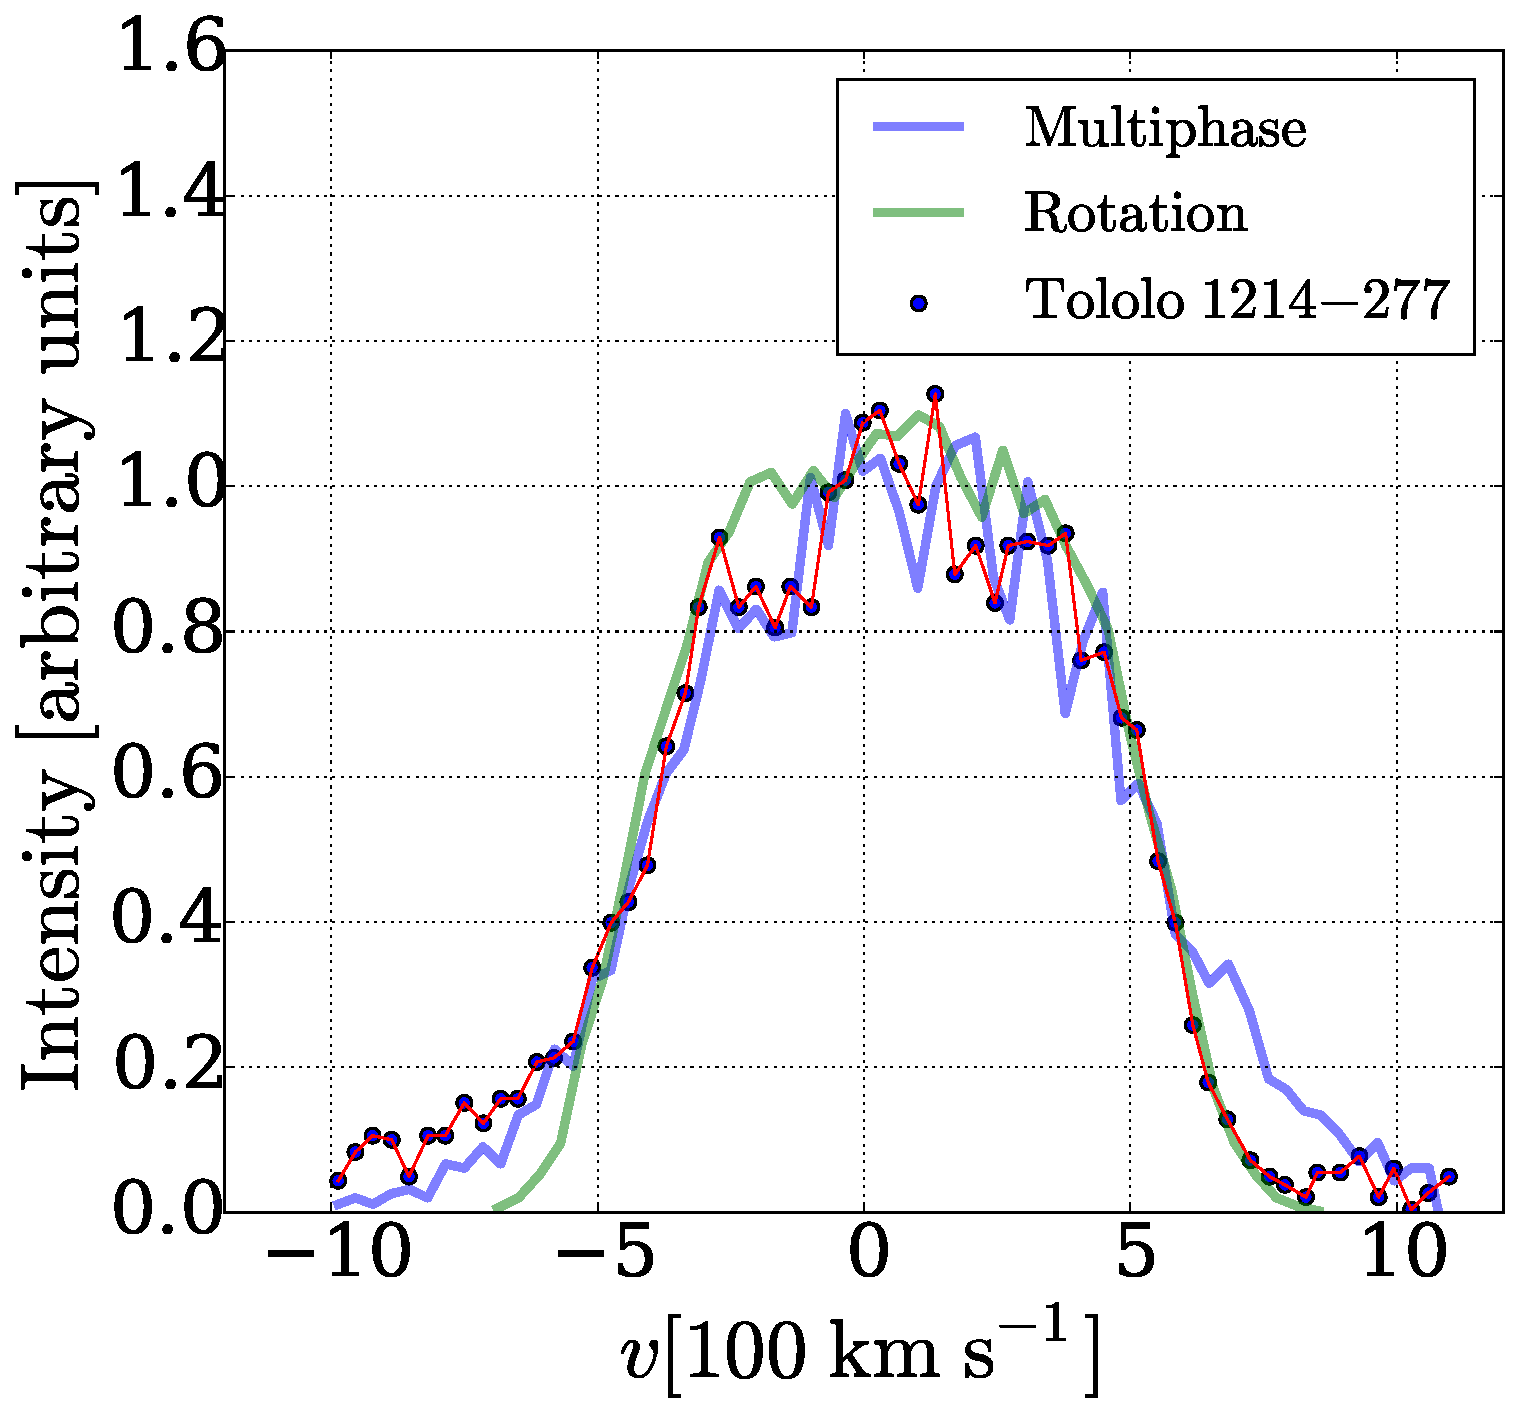
\includegraphics[width=0.6\textwidth]{CLARA-TOL-main.pdf}
\caption{Broad, single peaked and symmetric Ly-$\alpha$ emission of \tol.
  Dots correspond to the observational data. The line shows the results
of our best model from a full radiative transfer simulation both for
the rotation and multiphase models.} 
\end{center}
\end{figure*}

\begin{figure*}
\begin{center}
  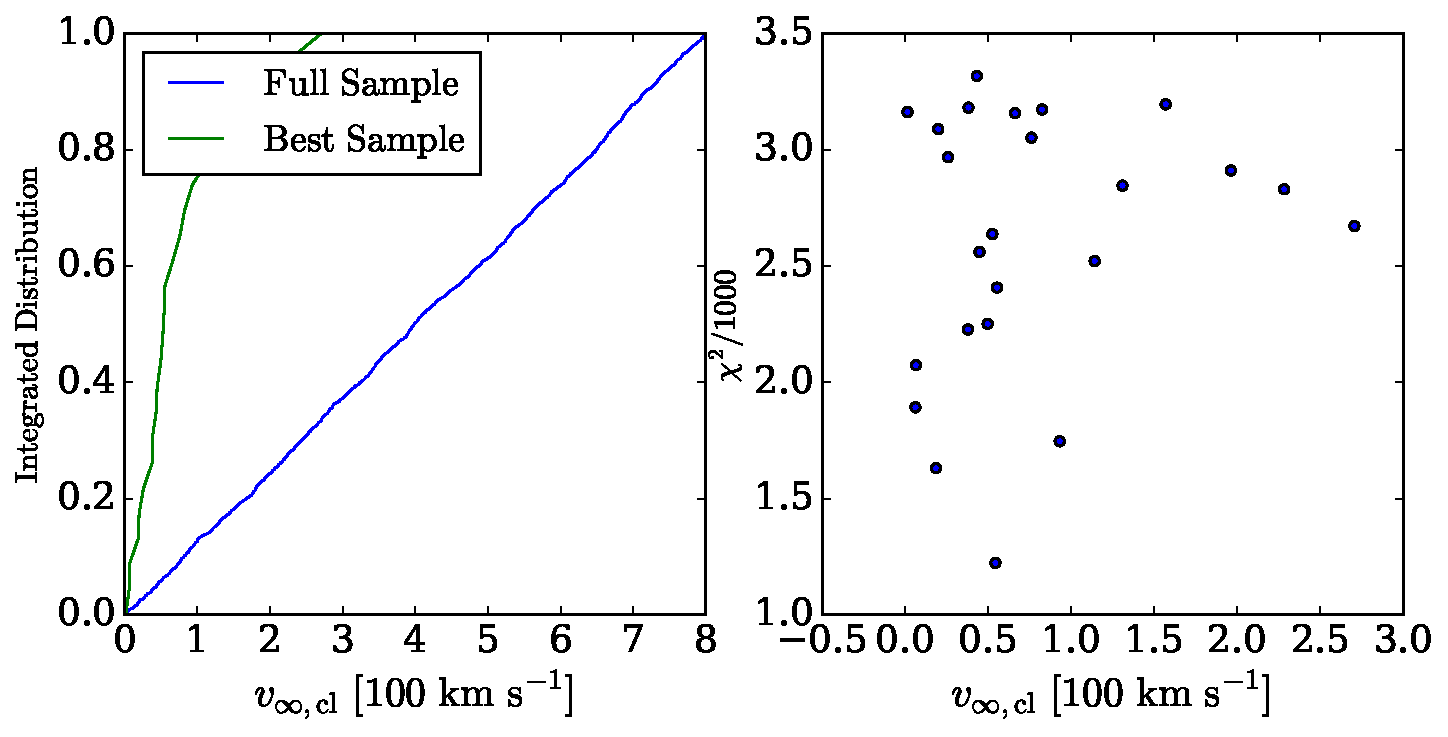
\includegraphics[width=0.6\textwidth]{vinf_cl.pdf}
  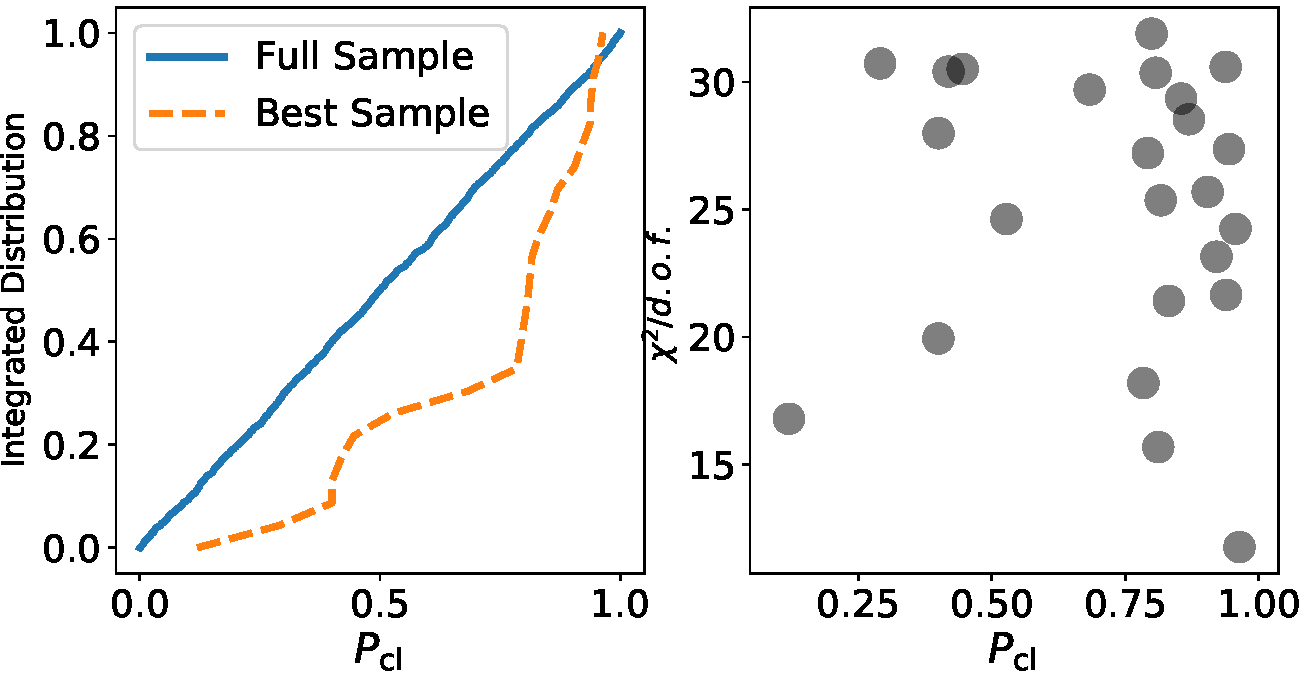
\includegraphics[width=0.6\textwidth]{P_cl.pdf}
  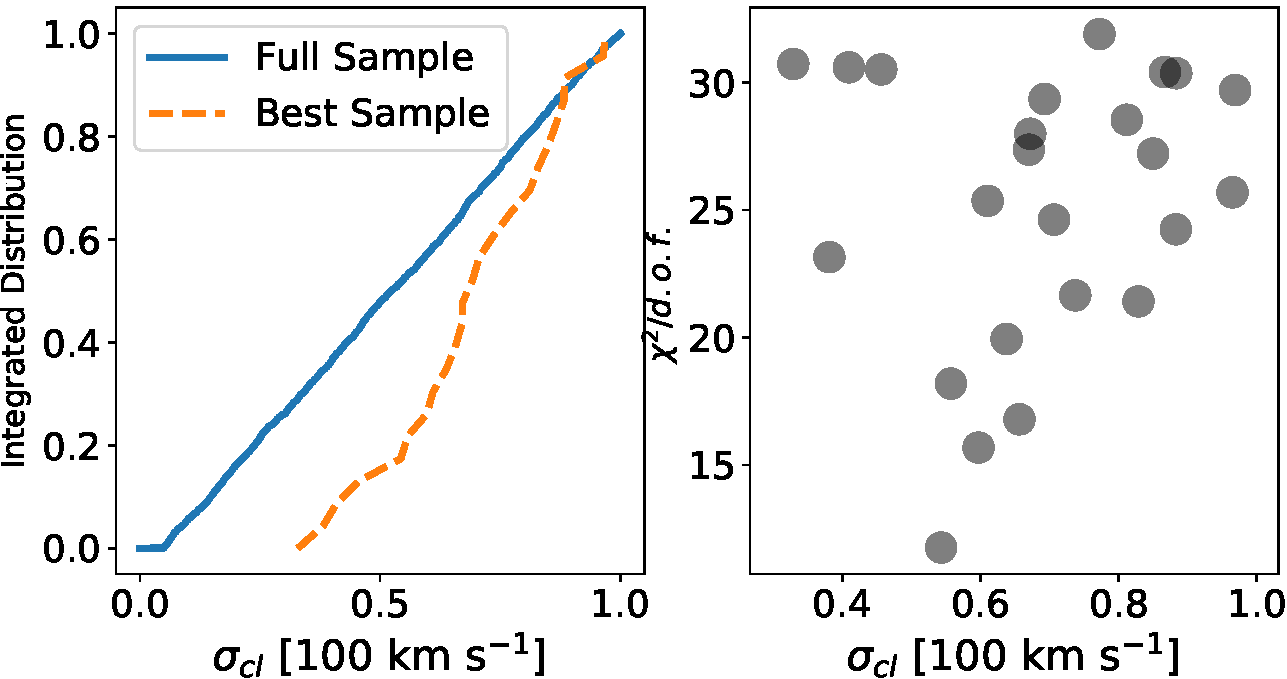
\includegraphics[width=0.6\textwidth]{sigma_cl.pdf}
\caption{Results from the multiphase
  model\label{multiphaseresults}.
  The left column corresponds to the parameter's integrated distributions for
  models with the lowest $\chi^2$ values (dotted line) compared against the
  parameter's integrated distributions (continous line) used as a prior.
  These are the only three parameters that show a significant statistical difference from
  the prior distributions, for all the other eleven parameters we
  cannot find any significant difference.}  
\end{center}
\end{figure*}

\begin{figure*}
\begin{center}
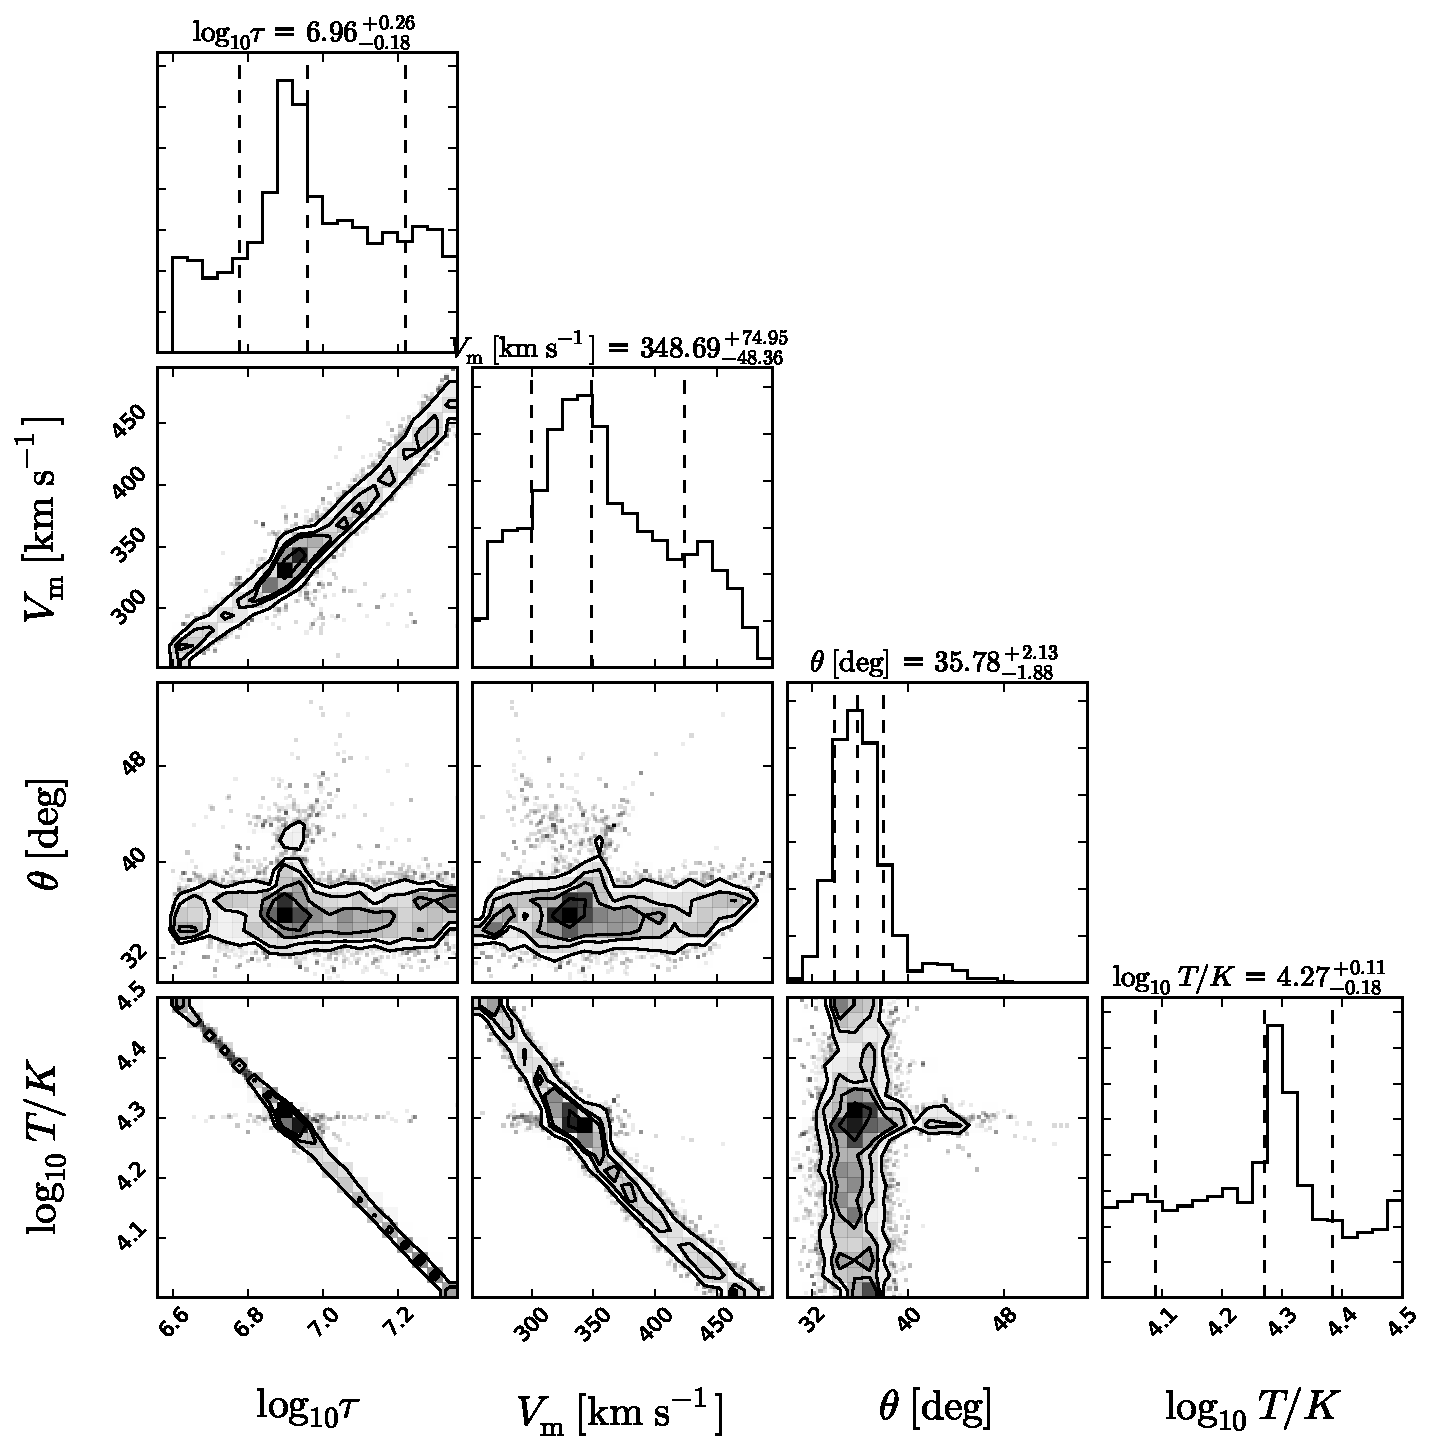
\includegraphics[width=0.8\textwidth]{emcee_results.pdf}
\caption{Results from the Markov Chain Monte Carlo computation for
    the rotation model. The dotted vertical lines in the outer histograms 
	represent the 16th, 50th and 84th percentiles. \label{emceeresults}} 
\end{center}
\end{figure*}


\section{Theoretical Models and Parameter Exploration}


\subsection{Multiphase ISM} 

The idealized multiphase model consists of spherical, cold, dens
clumps of neutral hydrogen (and dust) embedded in a hot, ionized
medium. 
The clumps also have a random and an outflowing velocity
component which totals the number of parameters describing the model
to be $14$.  {\bf These parameters are: MAX}

In order to map out this large parameter space, we randomly drew
$2500$ sets of parameters within a observationally realistic range
(based on the considerations of \citep{Laursen2013ApJ...766..124L})
yielding a large variety of single-, double- and triple-peaked
spectra. 
The full analysis of the the spectral features as well as
more details on the radiative transfer are presented in
\citep{Gronke2016}.    

We compare each resulting spectra to the observational results from
\tol\ after normalizing the observed and simulated spectra to have a a
flux integral of one.
We then build a $\chi^2$ on the normalized flux measurements for each one
of the $2500$ models, and then select for further analysis the best
$1\%$ models according to the lowest $\chi^2$ values.
The
$\chi^2$ gap in those $25$ models is close to $3000$, the lowest
$\chi^2$ being close to $1200$.
The total number of degrees of freedom is
$104$.    


Then we performed a Kolmogorov-Smirnov test to compare each parameter
distribution in the best $25$ models against the parent distribution
of $2500$ models. 
If we obtain a p-value $<0.05$ for a given model parameter, we conclude that
this parameter does influence the $\chi^2$ fit, as the distribution for
the best $\chi^2$ models is statistically different to the
distribution from the global sample of $2500$ models.  

The best values for the influential parameters correspond to
the values that produce the minimum
$\chi^2$.
The 1-$\sigma$ uncertainty comes from a parabolic fit to the
$\chi^2$ as a function of $v_{\infty,\rm{cl}}$, $\sigma_{\rm cl}$,
$P_{\rm cl}$ around its corresponding minimum.



\subsection{Bulk Rotation}

The rotation model corresponds to the work presented in
\citep{GaravitoCamargo2014} based on the Monte Carlo code
\texttt{CLARA} \citep{CLARA}. 
In that model the Ly-$\alpha$ photons are propagated 
within a spherical and homogeneous cloud of HI gas undergoing solid
body rotation.
The sphere is fully characterized by three parameters: the HI line's
center optical  depth $\tau$ measured from the center to its surface, the HI
temperature $T$, and the linear surface velocity $V_{\rm max}$.  
Including the effect of dust only changes the overall line
normalization but not its shape.  
The results we report do not include any dust model.
In this paper we use an analytical solution that captures the most
important effects of rotation onto the \lya\ line as explained by \citet{GaravitoCamargo2014}.


The analytical solution for the rotation sphere is the base to
perform the Markov Chain Monte Carlo (MCMC) calculation using the
\texttt{emcee} Python library \citep{2013PASP..125..306F}. \texttt{emcee} 
is an open source optimized implementation of the affine-invariant 
ensemble sampler for MCMC. 
The algorithm creates a number of walkers that,
during a sufficient number of steps, generate parameters' combinations
for a specific model. For each time, the code calculates the likelihood of the
combination with respect to the observational data. The walkers ecplore
the parameter space sampling the likelihood function.


\section{Results}


Figure 1. summarizes our findings.
Dots represent the observational data for \tol\ with the
overplot from our best fits from the analytical solution for a
urotating homogeneous gas sphere (thin line) and the multiphase
model (thick line). 


In spite of the simplicity of our models, this is the first time that
the main \tol\ features can be reproduced: a wide, centered,
single-peaked \lya\ line.
This result does not demonstrate that our models are unique to
reproduce \tol's features, but is a significant step forward to
understand why this source is atypical.


\subsection{Multiphase ISM}
Under these conditions we find $\sigma_{\rm cl}=$\sigmaclump,
$v_{\infty {\rm, cl}}=$\inftyclump\ and $P_{\rm cl}=$\probaclump. 

From this test we found that only three parameters influence the
$\chi^2$: the clump outflow velocity $v_{\infty,\rm{cl}}$ (p-value 
$10^{-18}$), the clump velocity dispersion $\sigma_{\rm cl}$ (p-value
$10^{-4}$) and the probability that the \lya\ emission comes from the
clumps $P_{\rm cl}$ (p-value $10^{-4}$). This does not mean the other
parameters do not influence the resulting spectra at all; it means
that they cannot be constrained from \tol's observations. 


Qualitatively as \tol\ possesses a very wide spectrum which can be
achieved by subsequent scatterings off (relatively) fast moving clumps
while the multi-phase nature (i.e., the existence of low-density
channels) ensures the high flux at line center as observed.     

\subsection{Bulk Rotation}

MCMC methods are optimal for sampling parameters at a high number of 
dimensions. In this case we explore flat priors on four parameters:
$200<V_{\rm max}/\mathrm{km\ s}^{-1} <600$,  
$6.0<\log_{10}\tau<9.0$, $4.0<\log_{10} T/10^4\mathrm{K}< 4.5$ and
$0<\theta<90$ using $500$ steps with $24$ walkers for a total of
$12000$ points in the chain. 
The results are summarized in 
Figure \ref{emceeresults}. 
From this model we find that the fiducial 
parameters that could explain the broad features in \tol\ are 
$V_{\rm max}=348^{+75}_{-48}$ km s$^{-1}$, $\log \tau = 6.96^{+0.26}_{-0.18}$, 
$\log_{10} T/\mathrm {K} = 4.27^{+0.11}_{-0.18}$ and $\theta = 35.78^{+2.13}_{-1.88}$ 
degrees.


The best parameters in the rotation model are a rotational velocity of 
$V_{\rm max}=348^{+75}_{-48}$ \kms, a neutral Hydrogen optical depth of 
$\log_{10}\tau=6.96^{+0.26}_{-0.18}$,  and an inter-stellar medium temperature of $\log_{10} T/\mathrm {K} = 4.27^{+0.11}_{-0.18}$.  
This model is also able to constrain the angle between the plane
perpendicular to the rotation axis and the observational line-of-sight
to $\theta = 35.78^{+2.13}_{-1.88}$ degrees.










\section{Discussion}

Having constrains for  velocity dipersion $\sigma$ of some dynamical
tracers (clumps in the case of the multiphase model) in a spherical
system located in a region of size $r$ we estimate the dynamical mass
within $r$. 


\begin{equation}
M_{\rm dyn} = 3 \frac{\sigma ^{2}r}{G} = 3.48\times10^{9}
\left(\frac{\sigma}{100\ \mathrm{km\ s}^{-1}}\right)^2\left(\frac{r}{\mathrm{kpc}}\right) M_{\odot}
\end{equation}

We use the 3D half-luminosity
radius, $r_{s}$, as the typical size for the HI region. 

In the case of rotational velocity $v$ in a region of size $r$ we
estimate the dynamical mass by 

\begin{equation}
M_{\rm dyn} = \frac{v ^{2}r}{G} = 1.16\times10^{9}
\left(\frac{v}{100\ \mathrm{km\ s}^{-1}}\right)^2\left(\frac{r}{\mathrm{kpc}}\right)M_{\odot} 
\end{equation}


In the multiphase model the best constrained parameters by the
observational data are the clump velocity dispersion
$\sigma_{\rm{cl}}=$\sigmaclump ,  the clump's outflowing velocity
$v_{\infty, \rm{cl}}=$\inftyclump\ and the fraction of the
\lya\ emission that is  coming from the cold clumps  $P_{\rm cl}=$\probaclump.


Assuming that the clumps are located in a spherical region of radius
$r_s=2.25$ kpc (corresponding to \tol's estimated 3D half-luminosity
radius), 
this corresponds to dynamical masses of $M_{\rm dyn} =
3.2_{-1.0}^{+1.6}\times 10^{10} M_{\odot}$ and $M_{\rm
  dyn}=2.31\pm0.04 \times 10^{9}$ $M_{\odot}$ for the
rotation and multiphase models, respectively, 

\tol's stellar mass is  $M_{\star} = 1.45\pm0.45\times 10^{8}
M_{\odot}$   \citep{2014PASP..126.1079M} and its total neutral HI mass is $M_{\rm HI}<2.65\times 10^{8}$ M$_{\odot}$. 
\citep{pustilnikmartin07}; the dynamical mass is at least 12 to 160 times
the baryonic mass, depending if one considers the multiphase or
rotation estimate. 

We lean towards the lower dynamical mass estimate from the multiphase
model as it seems easier to reconcile with the following two
astrophysical mechanisms for its origin.
The first way to explain a dynamical mass of $10^{9} M_{\odot}$
in a sphere of 2.25 kpc in radius, could be a dark matter halo of at
least $10^{12}$ M$_{\odot}$ in mass \citep{2011ApJ...726..108T}, which
leaves open the question as to why  \tol\ is not more similar to the
Milky Way galaxy as it would be hosted by a dark matter halo of similar
mass. 
A second possibility is that \tol\ hosts a supermassive black hole of
$10^{9} M_{\odot}$. This is almost two orders of magnitude higher
than the supermassive black hole found in the compact dwarf galaxy
M60-UCD1 \citep{2014Natur.513..398S}, which has a similar stellar mass
as \tol. This would leave open the question about the formation
process of such a system.   
 
Another perspective to appreciate the atypically high dynamical mass
estimates comes from the observed scaling relations for dwarf
galaxies.
Assuming that \tol\ followed the fundamental plane relationship
between its mean surface brightness $I_e$, the projected half-light
radius $R_e$ and the velocity dispersion $\sigma$, described by $\log
I_e=1.6 \log\sigma - 1.21\log R_e + 0.55$ \citep{2009ApJ...698.1590G},
the expected velocity dispersion should be on the order of $5 \pm 1$ 
\kms, which is a factor of $\sim$ $10$ - $60$ lower than the 
results from the multiphase and rotation models, respectively. 
These are equivalent to factors of $\sim$ $100$ - $3600$ on the
dynamical mass.
Once again,  \tol\ seems to be significantly more massive than
expected. 



\section{Conclusions}

In this paper we presented two theoretical models that explain the main
observational feature of \tol, which have been unexplained so far.
One model is based on a multiphase ISM and the other on gas rotation,  
It is the first time that an observed \lya\ profile can be fully
reproduced by either of these two conditions.
Furthermore, the kinematics of both models suggest a dynamical mass
ten times larger than the baryonic mass infered from observations.

A new observational test is needed to clarify the physical nature of
\tol. 
We suggest that integral field unit measurements spatially
resolving its spatial extent are up to the task. 
\tol\ spans a region of $4$ arcseconds,
an instrument such as the Multi Unit Spectroscopic Explorer
\citep{2014Msngr.157...13B} with its
nominal $0.2$ arcseconds spatial sampling over a $1.0$ arcminute field
in wide-field mode could provide a coarse mapping of different
ionization lines to infer a kinematic map.
Another observational test includes the measurement of the
\lya\ ionizing continuum escape fraction.
In the rotational model this fraction should be zero, while
the multiphase model predicts that averaging over all sightlines
it should be around $0.5^{+1.0}_{-0.4}$\%, with the possibility of strong
variations depending on viewing angle \citep{2014MNRAS.444.1095G}. 

All in all, the mere existence of a strong LAE galaxy with a broad,
symmetric line is interesting.
It raises the question whether some high redshift LAEs have asymmetric
lines because the blue half was truncated by the intergalactic medium.
In this case the \lya\ radiation could emerge as a low surface
brightness glow, which may be connected to \lya\ halos, while also
influencing the way LAEs can be used as a probe of reionization
\citep{2014PASA...31...40D}.  

These findings demonstrate the importance of including rotation and multiphase
conditions as features to model the \lya\ line in high redshift
galaxies.
Additionally, if the hypothesis of a supermassive black
hole in \tol\ proves to be consistent with future observational
kinematic maps, it could correspond to a so far undetected
supermassive black hole in a dwarf galaxy, providing a new way to test
and probe theories on the co-evolution of galaxies and black holes in
the first generation of galaxies.   



\section*{Acknowledgments}

\bibliographystyle{mn2e}
\bibliography{references}

\end{document}

